%! TEX root = **/010-main.tex
% vim: spell spelllang=en:

\section{Performance analysis and optimizations}

\Cref{fig:time_cuda} shows a comparison of the execution time of the initial
implementation of the CUDA version against the sequential version when
calculating the diameter of the cycles. For this benchmark $10^4$ steps were
performed on each trajectory.  We can observe that the execution time
in CUDA for 1 to $2^{14}$ trajectories is roughly the same but past this point the
time starts to increase at a ratio similar to the sequential code.


\begin{figure}[H]
    \centering
    \includegraphics[width=1.0\textwidth]{figures/plots/time.tikz}
    \caption{Execution time of CUDA version vs. Sequential \\ (Diameter
    calculation)}%
    \label{fig:time_cuda}
\end{figure}

\begin{figure}[H]
    \centering
    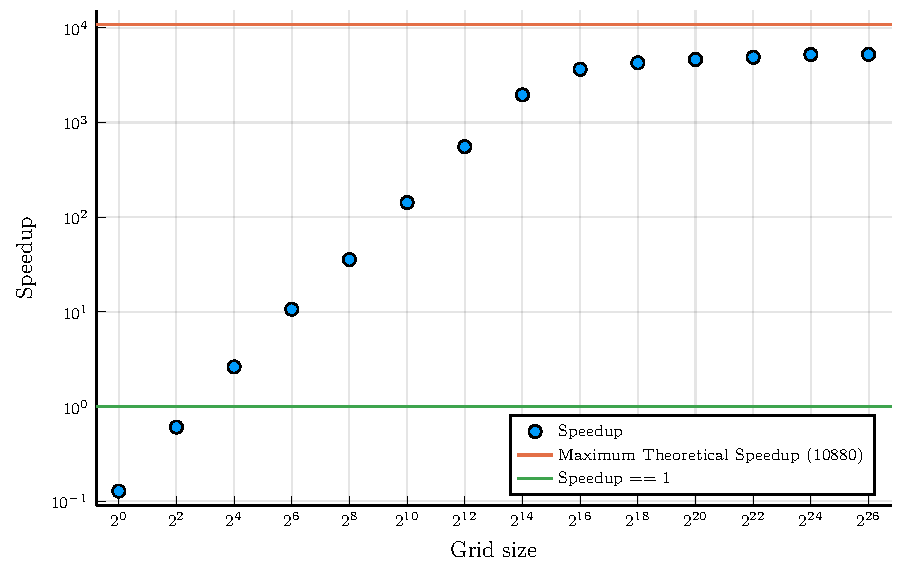
\includegraphics[width=1.0\textwidth]{figures/plots/speedup.tikz}
    \caption{Speedup of CUDA version vs. Sequential \\ (Diameter
    calculation)}%
    \label{fig:speedup}
\end{figure}

If we analyze the speedup obtained from the data (shown in \cref{fig:speedup})
we can see how the speedup reached is around $10^3$ from a theoretical maximum
on this GPU of $10240$. There is still an order of magnitude from the maximum
achievable speedup which gives room for improvement. Specially if we use
additional GPUs. For reference, the computation of $2^{22} \approx 10^6$ trajectories
took 4.284s on the GPU while the sequential version of the program takes around
40 minutes.
